\section{Acronyms Used}
\label{sec:acronyms}

\begin{acronym}[WWW] % Give the longest label here so that the list is nicely aligned
    \ifthenelse{\boolean{review}}
        {}
        {\acro{VMD}{Virtual Moderation Dataset}}
    
	\acro{LLM}{Large Language Model}
	\acro{ML}{Machine Learning}
	\acro{RL}{Reinforcement Learning}
	\acro{SDB}{SocioDemographic Background}
    \acro{AQ}{Argument Quality}
    \acro{CeRI}{Cornell e-Rulemaking Initiative}
    \acro{nDFU}{normalized Distance From Unimodality}
    \acro{OLS}{Ordinary Least Squares}
    \acro{GPL}{GNU General Public License}
\end{acronym}


\section{Methodological Details}

\subsection{Synthetic Discussion Generation}
\label{ssec:appendix:discussion}

An overview of how the experiments are generated can be found in Algorithm~\ref{alg:exp_generation}. We provide our framework with a set of starting opinions (``seed opinions'') and \acp{SDB}. We then run $N_d=8$ discussions for each pair of facilitation strategies $S$ and model. Synthetic generation is then handled as described in \S\ref{sec:methodology}. We use the \texttt{transformers} library to load and manage the model.

\begin{algorithm}[ht]
\caption{Synthetic discussion setup generation}
\label{alg:exp_generation}
\hspace*{\algorithmicindent} \textbf{Input:} 
         \begin{itemize}[noitemsep, nosep]
             \item User \acsp{SDB} $\Theta = \{\theta_1, \dots, \theta_{30}\}$
             \item Moderator \acs{SDB} = $\theta_{mod}$
             \item Strategies $S = \{s_1, \ldots, s_6\}$
             \item Seed opinions $O = \{o_1, \ldots, o_7\}$
             \item \acp{LLM} = $\{llm_1, llm_2, llm_3\}$
         \end{itemize}
         \hspace*{\algorithmicindent} \textbf{Output:} Set of discussions $D$
\begin{algorithmic}[1]
    \State $D = \{\}$
    \For{$llm \in LLMs$}
        \For{$s \in S$}
            \For{$i = 1, 2, \ldots, N_d$}
                \State $\hat{\Theta} = $ \Call{RandomSample}{$\Theta$, 7}
                \State $U =$  \Call{Actors}{llm, $\hat{\Theta}$}
                \State $m = $ \Call{Actors}{llm, $\{[\theta_{mod}, s]\}$}
                \State $o = $ \Call{RandomSample}{$O$, 1}
                \State $d =$ \{users: $U$, mod: $m$, topic: $o$\}
                \State $D = D \cup d$
            \EndFor
        \EndFor
    \EndFor
    \State \Return $D$
\end{algorithmic}
\end{algorithm}

\subsection{SocioDemographic Prompting}
\label{sssec:appendix:sdbs}

Table \ref{tab:sdb} shows the \ac{SDB} information provided to each synthetic participant. This applies to \ac{LLM} users, annotators and moderators. In ablation studes where we remove the \acp{SDB}, each value is replaced with the string “unknown”. The “Special Instructions” refer to the participant's role (\S\ref{sssec:appendix:roles}). The actual values used for each of the $30$ \ac{LLM} user-agents and $10$ annotator-agents and the moderator, can be found in the project's repository\analysislink.

\begin{table}
	\centering
	\begin{tabular}{|l|l|}
		\toprule
		Name & Type \\
		\midrule
		Username & string \\
		Age & integer \\
		Sex & string \\
		Education Level & string \\
		Sexual Orientation & string \\
		Demographic Group & string \\
		Current Employment & string \\
		Special Instructions & string \\
		Personality Characteristics & list of strings \\
		\bottomrule
	\end{tabular}
	\caption{\ac{SDB} information provided to the synthetic participants. Because of the size of the data instances, we defer the reader to the project repository for the actual values.\analysislink}
	\label{tab:sdb}
\end{table}


\section{Generalizing the Annotation Framework}

While toxicity is a reliable and important metric, we can also investigate other discussion quality dimensions, such as \ac{AQ}. \ac{AQ} is an important metric, frequently studied in the field of online facilitation \cite{argyle2023, schroeder-etal-2024-fora, falk-etal-2024-moderation, falk-etal-2021-predicting} and which can be correlated with toxicity \cite{chang-danescu-niculescu-mizil-2019-trouble}. However, it is also vague as a term; \citet{wachsmuth-etal-2017-computational} provide a definition comprised of logical, rhetorical, and dialectical dimensions, although other dimensions have also been proposed \cite{habernal-gurevych-2016-argument, persing-ng-2015-modeling}. Indeed, determining \ac{AQ} is a difficult task, since even humans disagree on what constitutes a ``good argument” \cite{wachsmuth-etal-2017-computational, argyle2023}. Nevertheless, in this section we present preliminary results obtained by prompting \ac{LLM} to measure \ac{AQ}(\S\ref{ssec:appendix:prompts}). 

Most findings w.r.t. toxicity are mirrored for \ac{AQ}. Fig.~\ref{fig:aq_stats} demonstrates that the presence of an \ac{LLM} facilitator qualitatively improves the \ac{AQ} of synthetic discussions, although to a lesser extent when compared with toxicity (c.f.\  Fig.~\ref{fig:toxicity_stats}). Similarly, there is no qualitative, observed improvement when advanced facilitation strategies are used (Fig.~\ref{fig:aq_stats}). \ac{LLM} users also show worse \ac{AQ} in the presence of trolls, when we use our specialized instruction prompt. Contrary to toxicity, the presence of \ac{LLM} facilitators does not seem to improve \ac{AQ} over time, as demonstrated in Table~\ref{tab:argq}.

\begin{figure}
	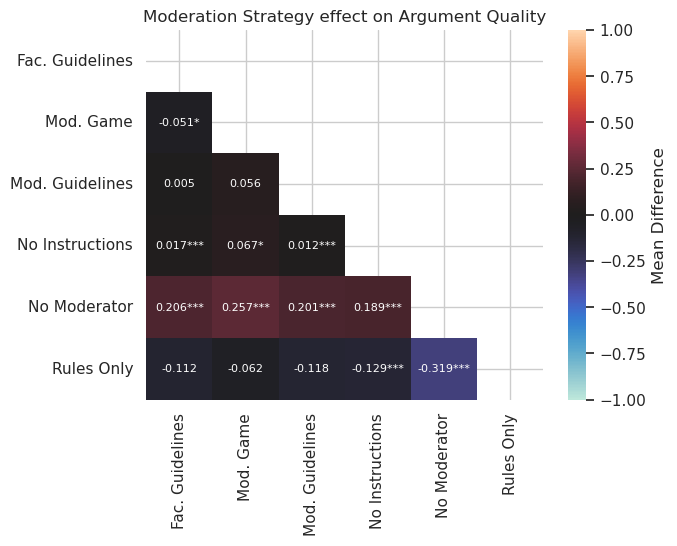
\includegraphics[width=\linewidth]{resources/argumentq_stats.png}
	\centering
	\caption{Difference in average \ac{AQ} levels for comments following pairs of facilitation strategies. When the value of a cell at row $i$ and column $j$ is $x$, strategy $i$ leads to overall more ($x>0$), or less ($x<0$) intense toxicity compared to $j$ for an average of $x$ points in a scale of $1-5$. For each comparison, we use a pairwise Student t-test; p-values shown as asterisks (\asterisknote).}
	\label{fig:aq_stats}
\end{figure}


\begin{table}
	\centering
	\begin{tabular}{p{5cm} p{1.5cm}}
		\toprule
		\textbf{Variable} & \textbf{Arg.Q.} \\
		\midrule
		Intercept & 2.113\textsuperscript{***} \\
		\strategynoinstr & -0.213\textsuperscript{***} \\
		\strategymodgame & -0.282\textsuperscript{***} \\
		\strategyrules & -0.305\textsuperscript{***} \\
		\strategyregroom & -0.107\textsuperscript{*} \\
		\strategyconstrcomm & -0.007\textsuperscript{} \\
		time & -0.012\textsuperscript{**} \\
		No Instructions$\times$time & 0.003 \\
		\strategymodgame$\times$time & 0.003 \\
		\strategyrules$\times$time & -0.002 \\
		\strategyregroom$\times$time & -0.011\textsuperscript{*} \\
		\strategyconstrcomm$\times$time & -0.024\textsuperscript{***} \\
		\bottomrule
	\end{tabular}
	\small
	\asterisknote
	\normalsize
	\caption{\ac{OLS} regression coefficients for Arg.Q. ($Adj.R^2=0.016$). \textit{“Time”} denotes dialogue turn, reference factor is \emph{\strategynomod}.}
	\label{tab:argq}
\end{table}


\begin{figure}
	\centering
	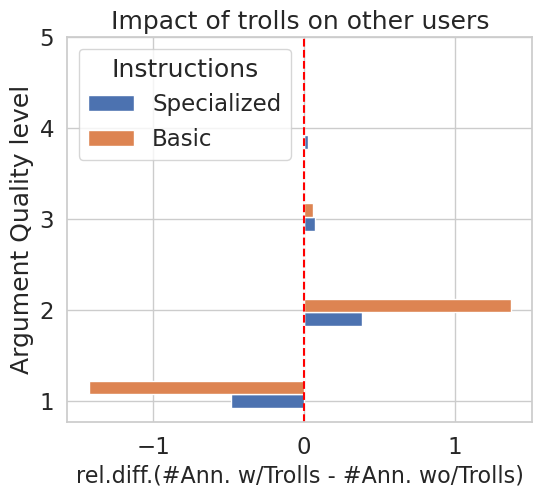
\includegraphics[width=0.8\linewidth]{aq_trolls.png}
	\caption{Relative differences in number of annotations per \ac{AQ} of synthetic discussions, when comments by troll users are excluded. We compare between our specialized and a basic instruction prompt.}
	\label{fig:aq_trolls}
\end{figure}



\section{Additional Analysis}

\subsection{The Role of Roles}

We verify that the models and roles used did not by themselves impact the findings presented in \S\ref{ssec:results:main}. Fig.~\ref{fig:toxicity_aq_role} demonstrates that, as expected, only troll user-agents contribute on average worse toxicity and \ac{AQ} in the synthetic discussions. Furthermore, Fig.~\ref{fig:toxicity_aq_model} shows that toxicity and \ac{AQ} are on average not qualitatively dependent on the model used.

\begin{figure*}
	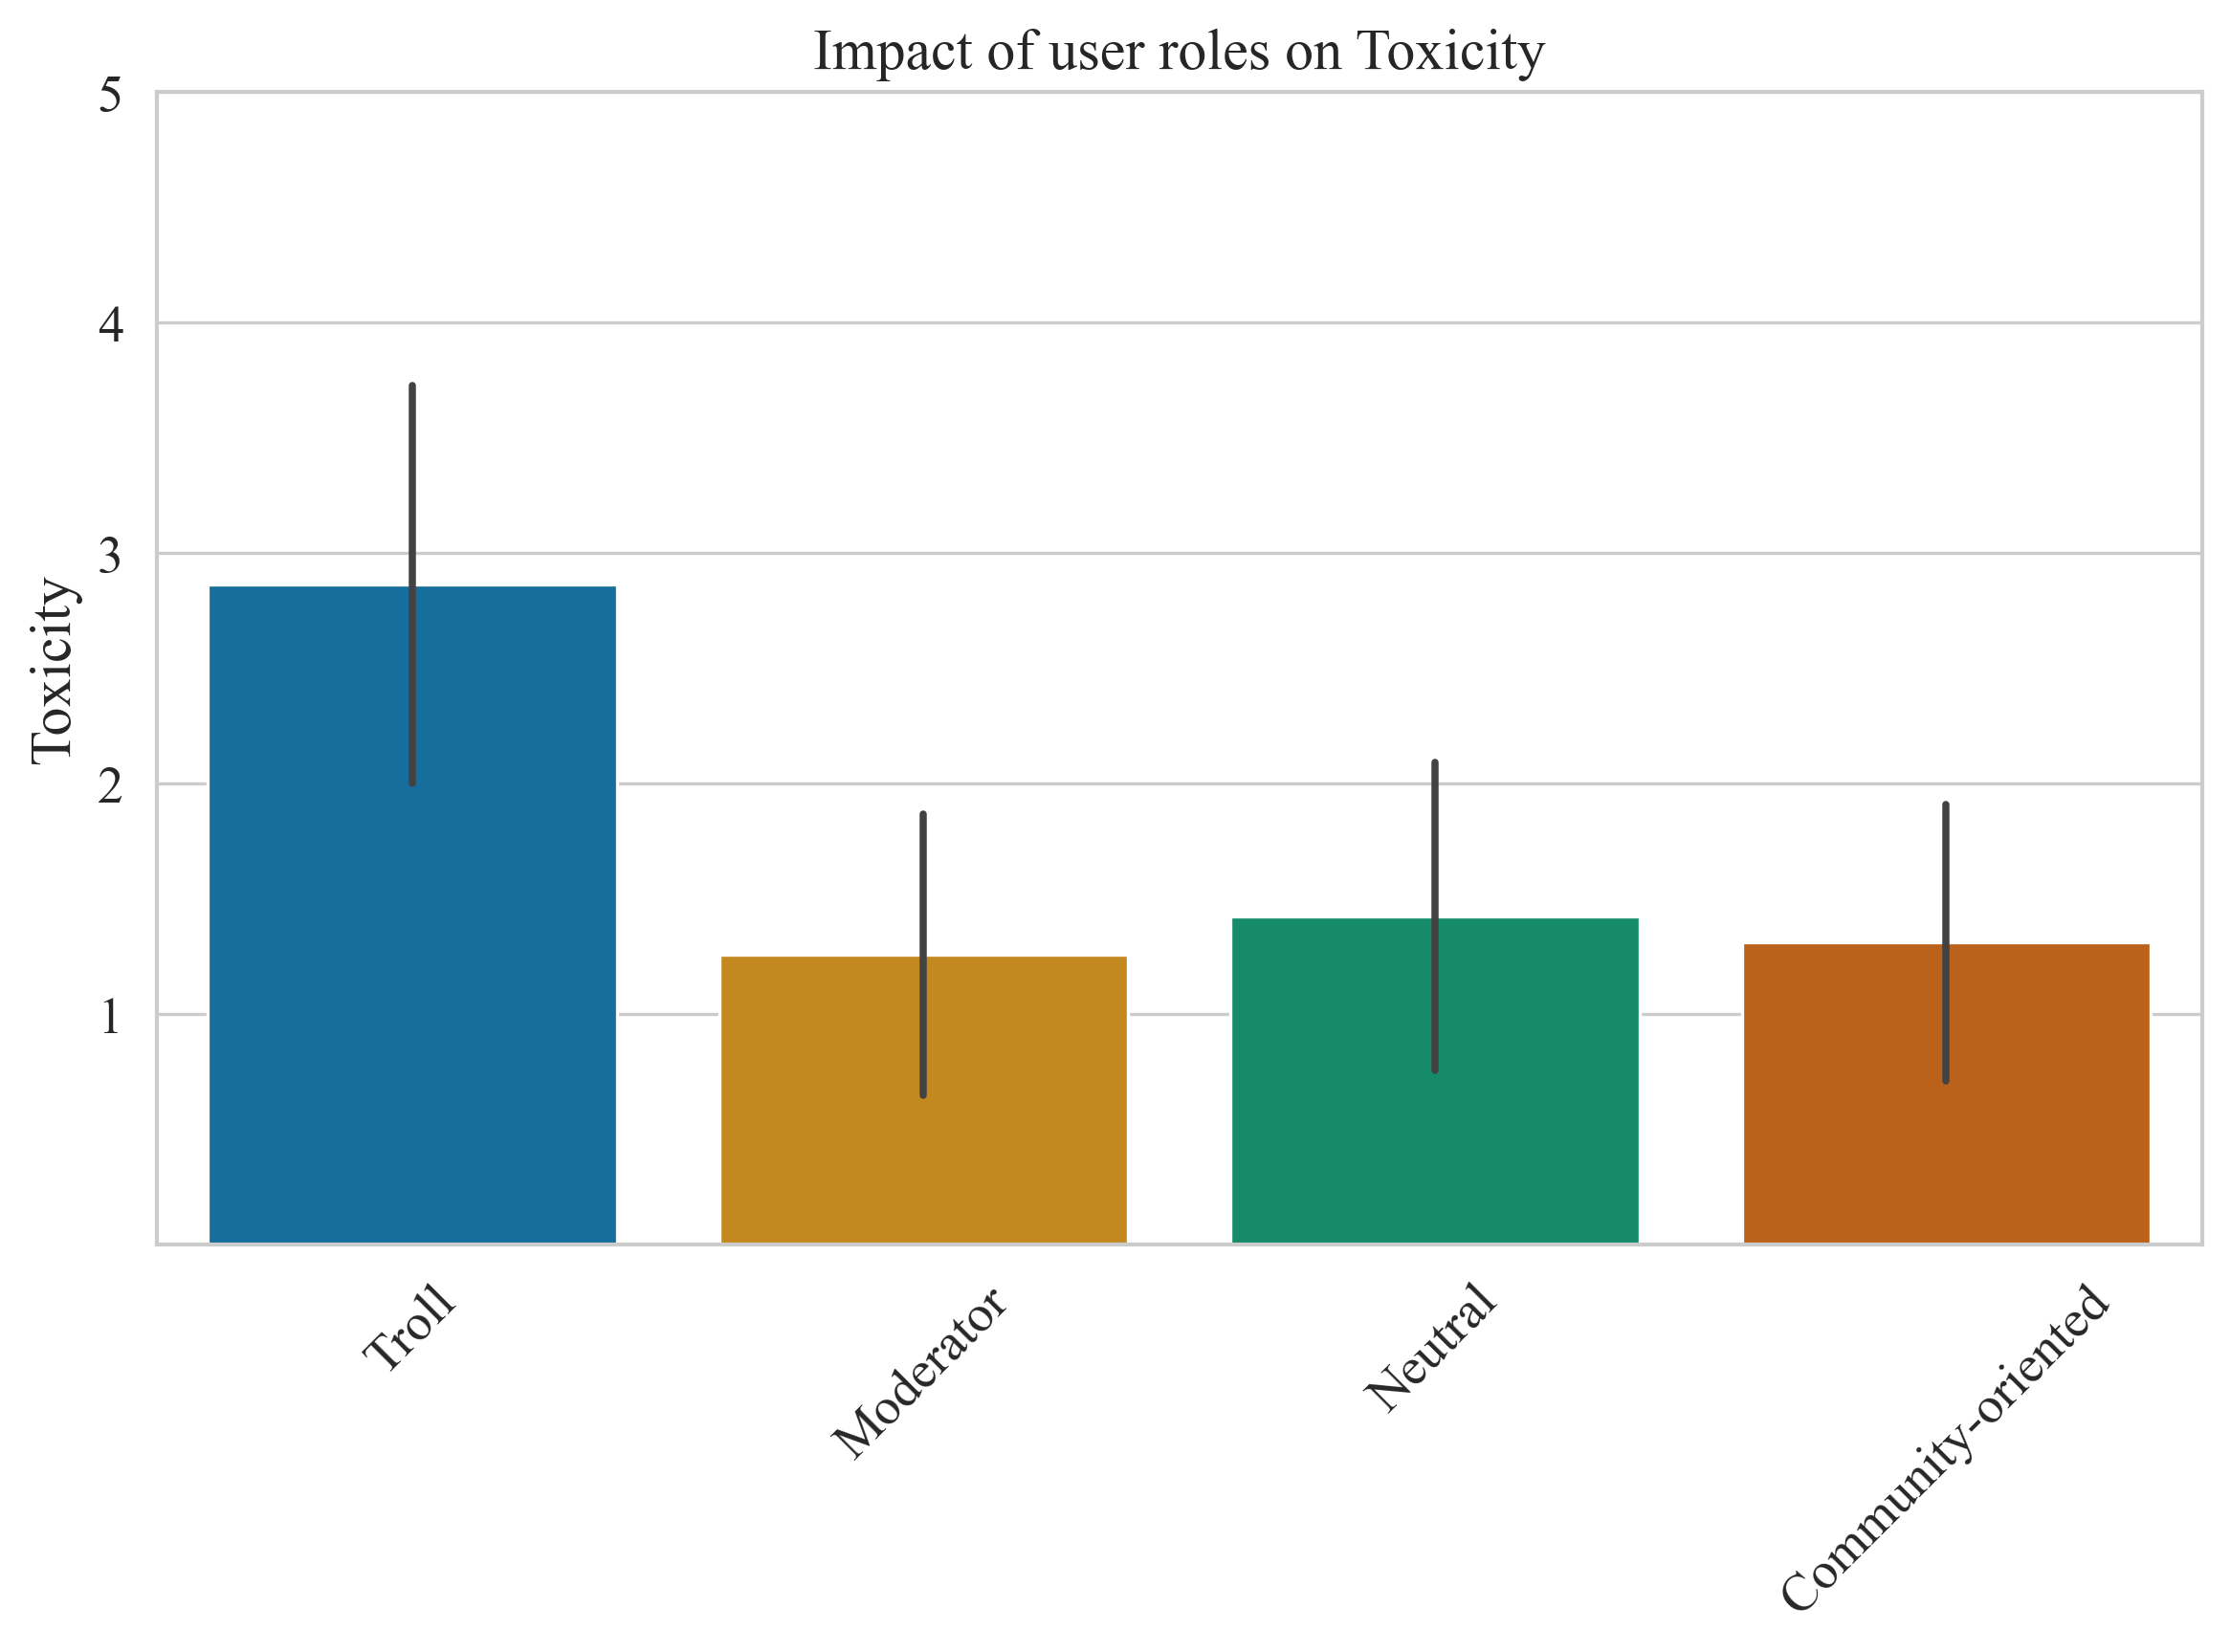
\includegraphics[width=0.45\linewidth]{toxicity_intent_barplot.png} \hfill
	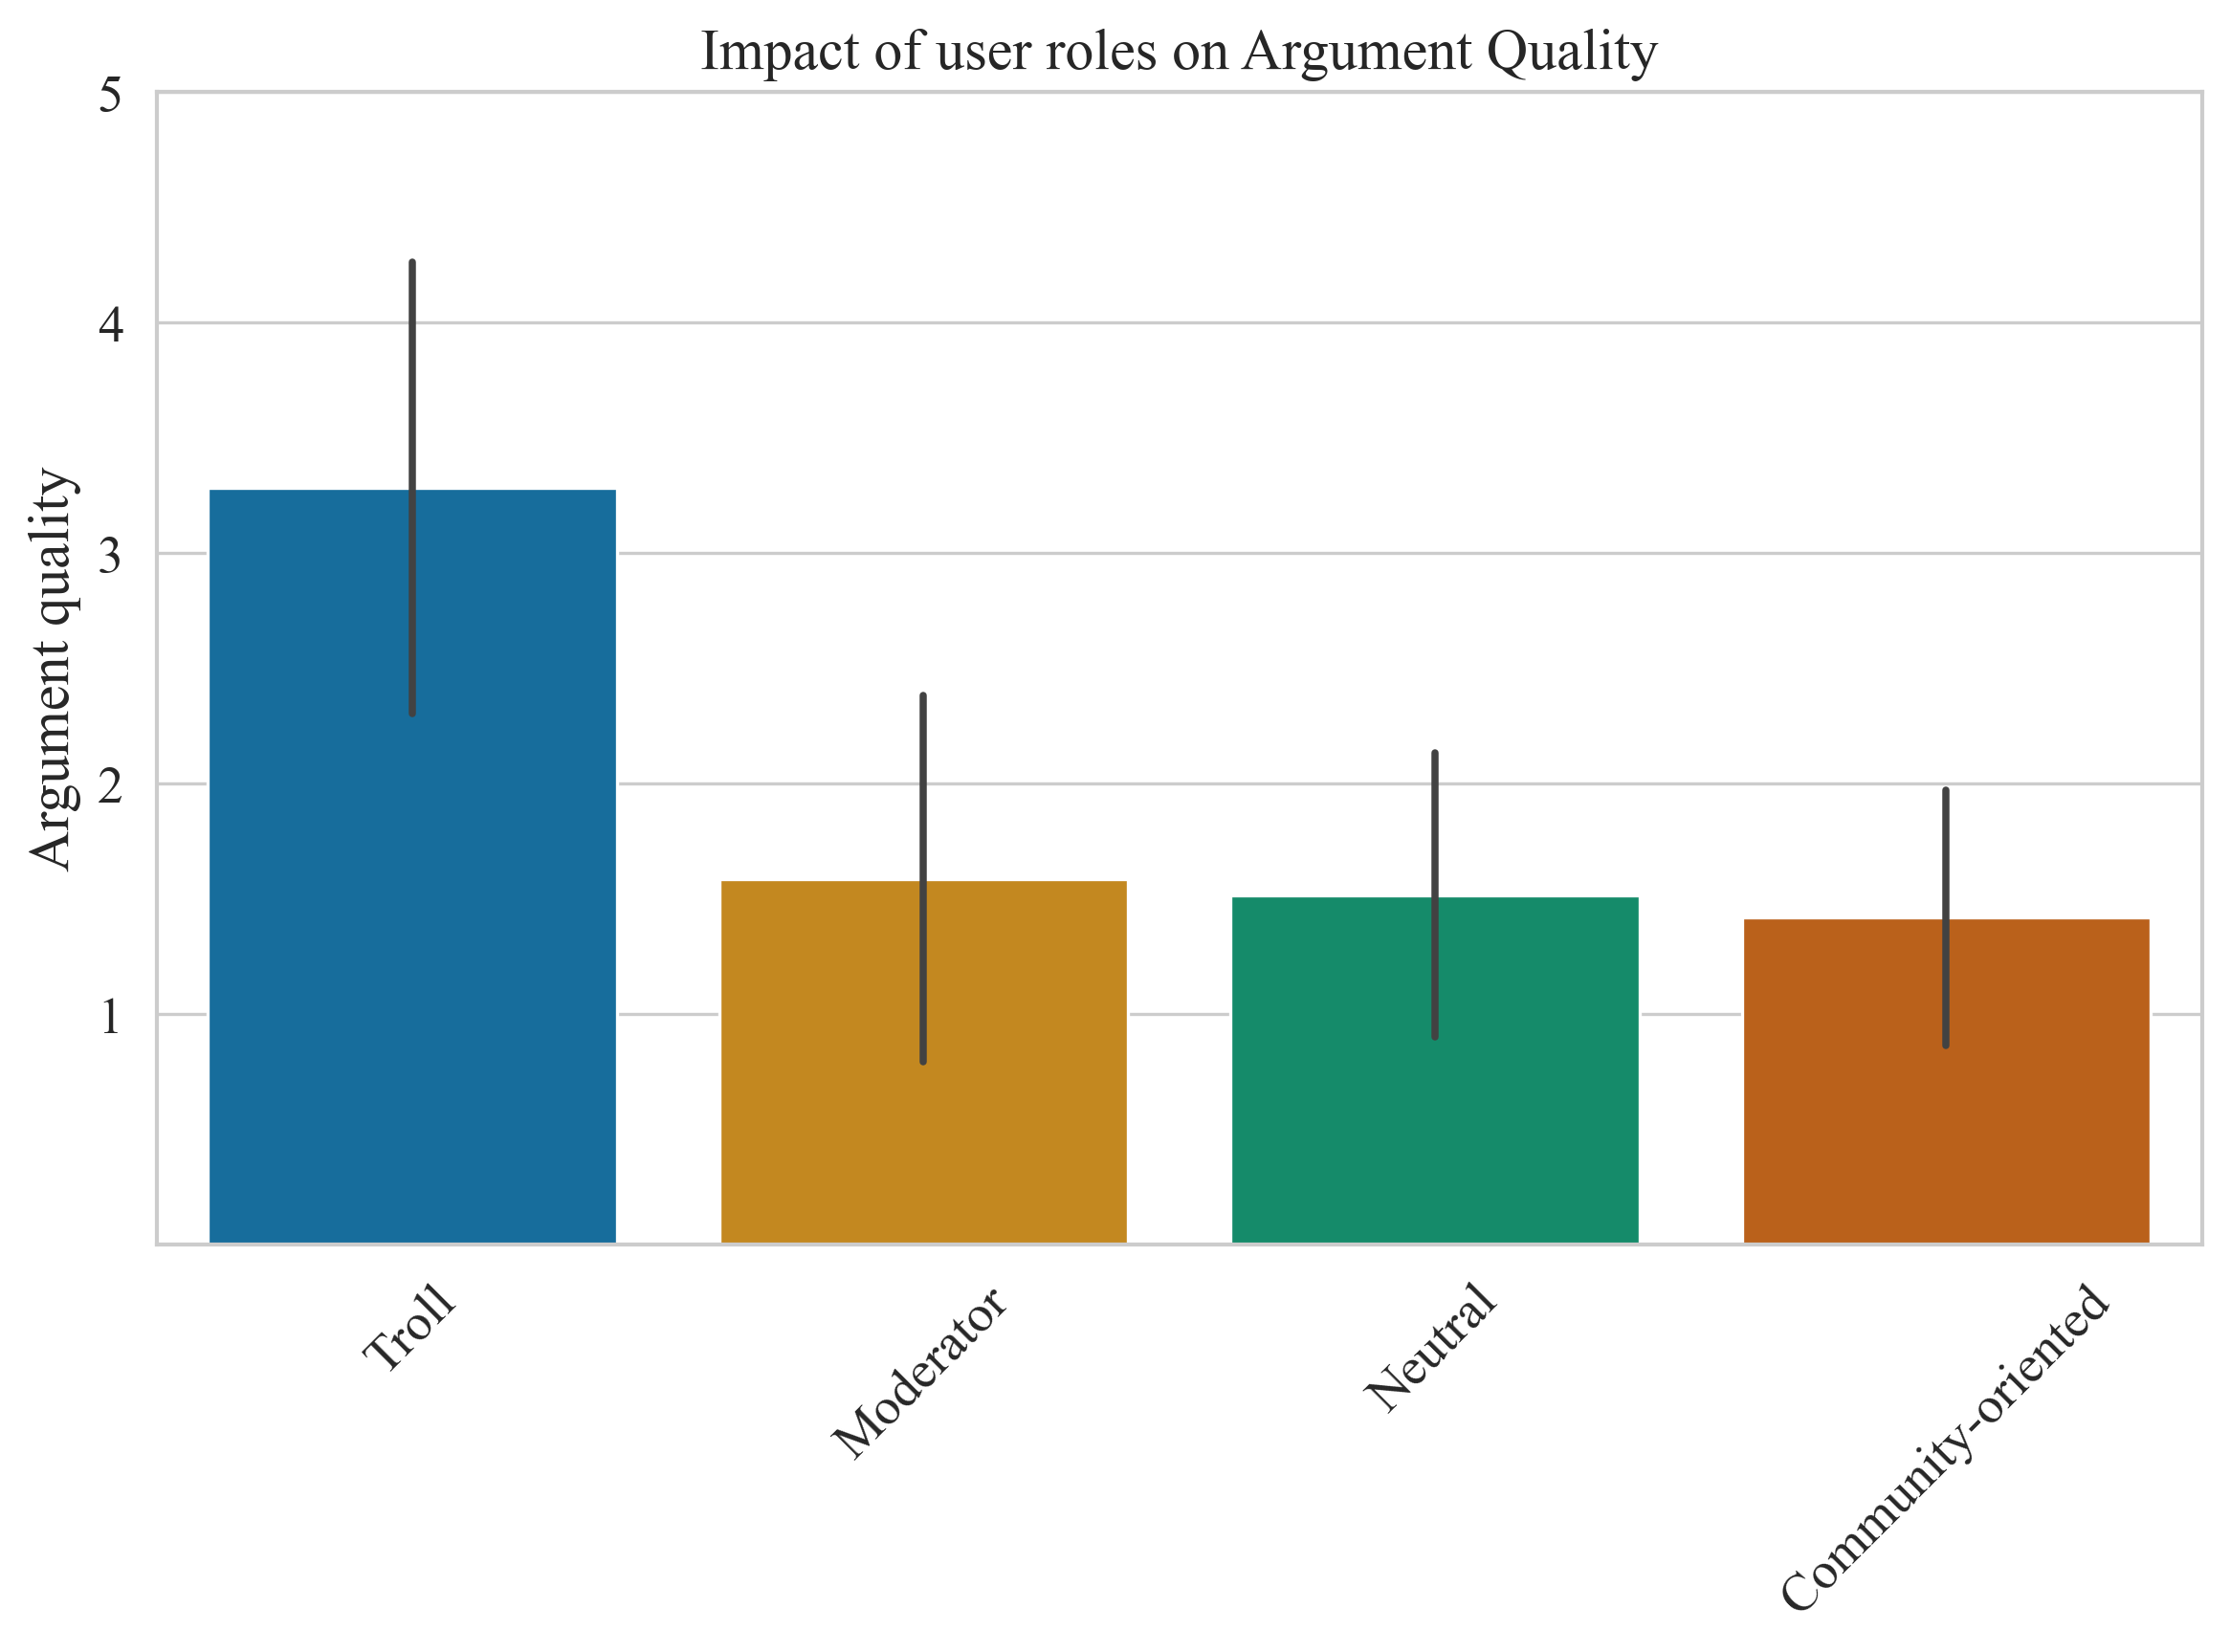
\includegraphics[width=0.45\linewidth]{aq_intent_barplot.png}
	\centering
	\caption{Average Toxicity (left) and \acf{AQ} (right) per \ac{LLM} user-role (\S\ref{ssec:methodology:prompts}).}
	\label{fig:toxicity_aq_role}
\end{figure*}

\begin{figure*}
	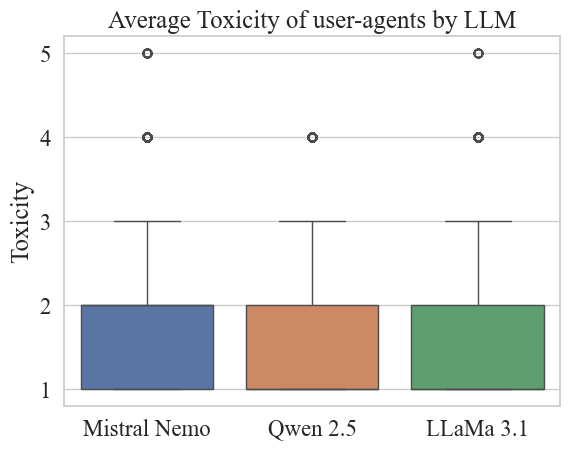
\includegraphics[width=0.45\linewidth]{toxicity_llm_barplot.png} \hfill
	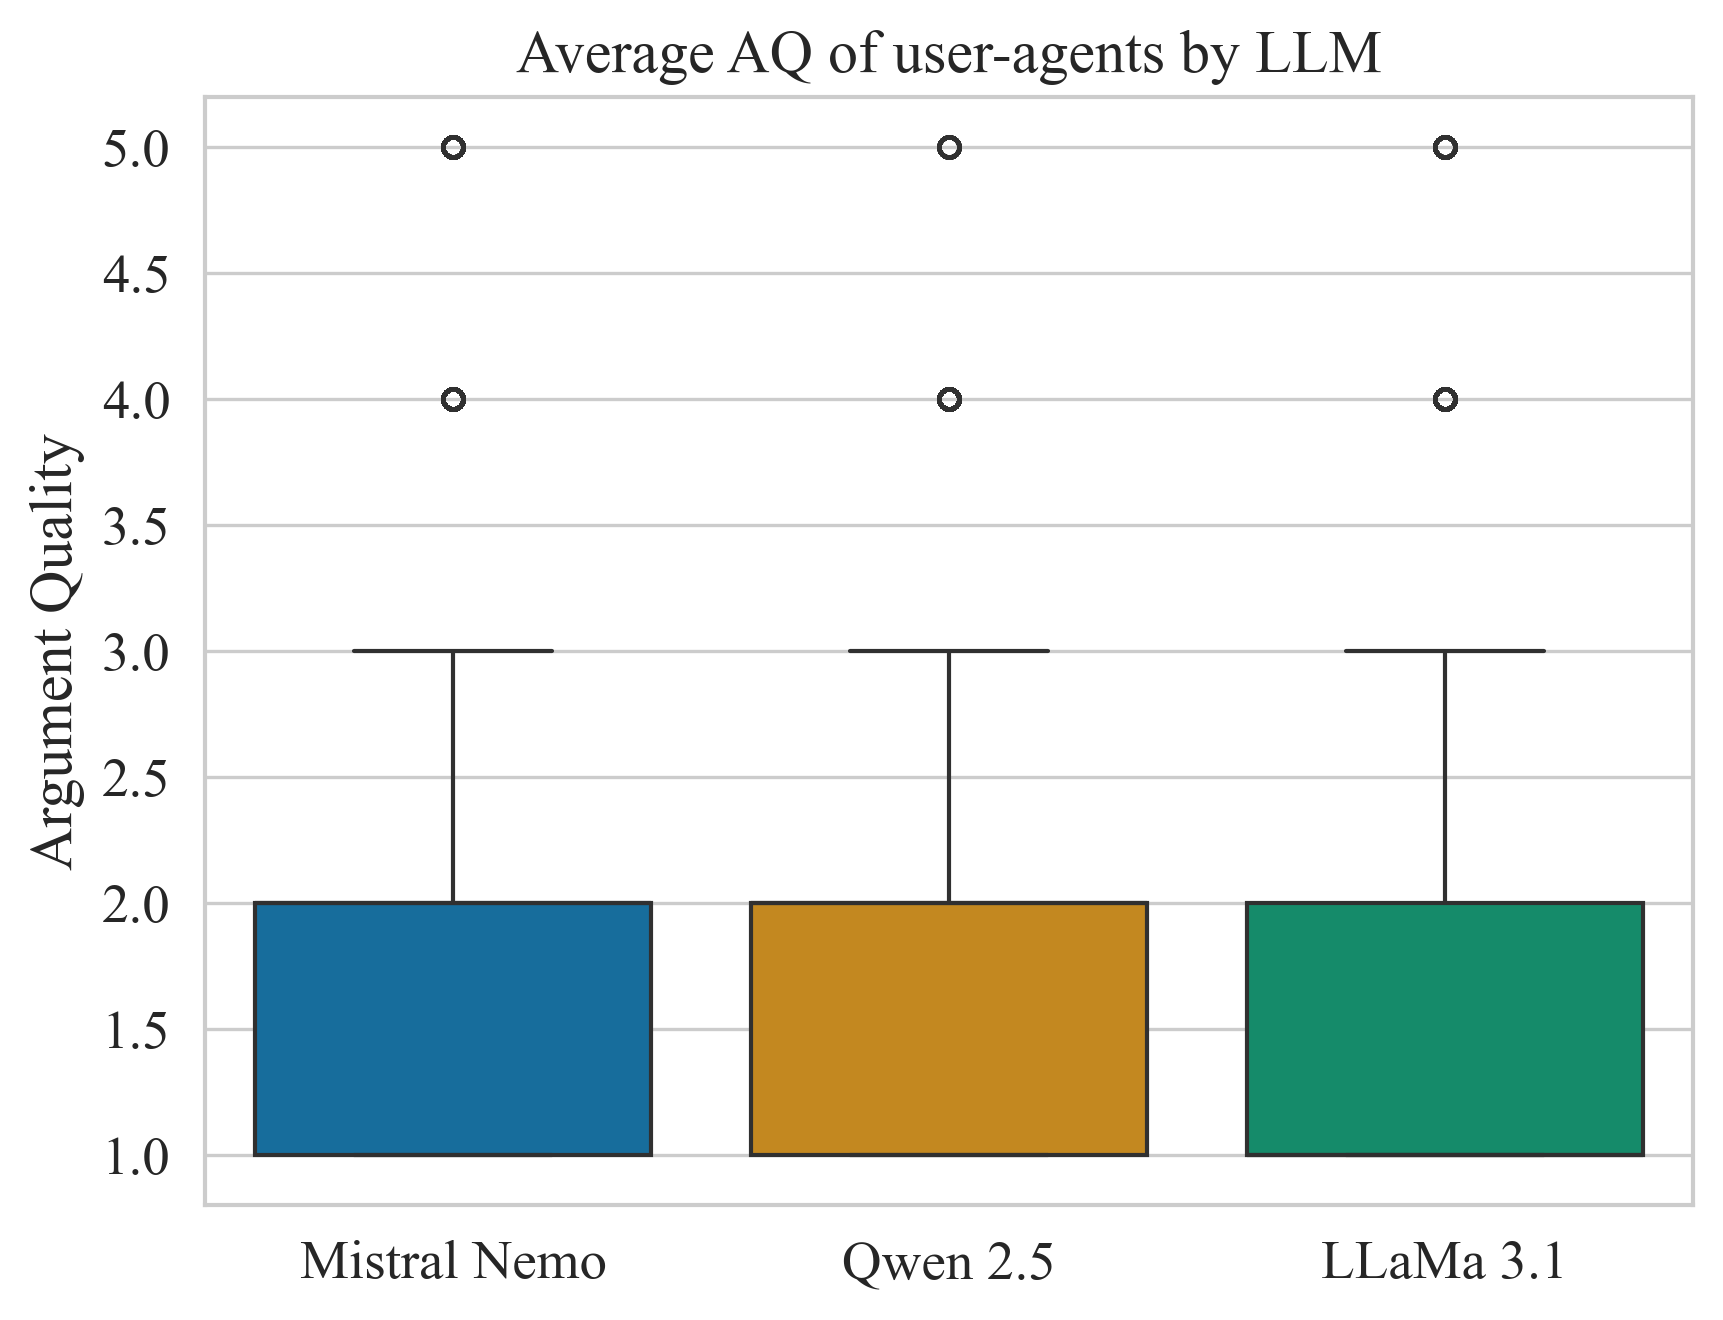
\includegraphics[width=0.45\linewidth]{aq_llm_barplot.png}
	\centering
	\caption{Boxplots for average Toxicity (left) and \acf{AQ} (right) per \ac{LLM} (\S\ref{ssec:experimental:setup}).}
	\label{fig:toxicity_aq_model}
\end{figure*}


\subsection{Comment Length}

\begin{figure*}[t]
	\begin{subfigure}{0.32\linewidth}
		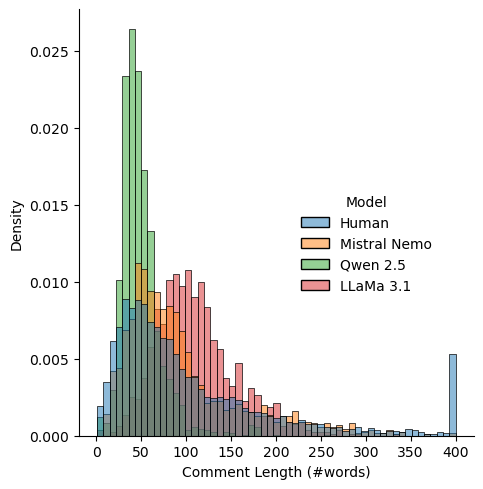
\includegraphics[width=\textwidth]{comment_len_model.png}
		\caption{Model}
		\label{fig:comment_length_model}
	\end{subfigure}%
	\hfill
	\begin{subfigure}{0.32\linewidth}
		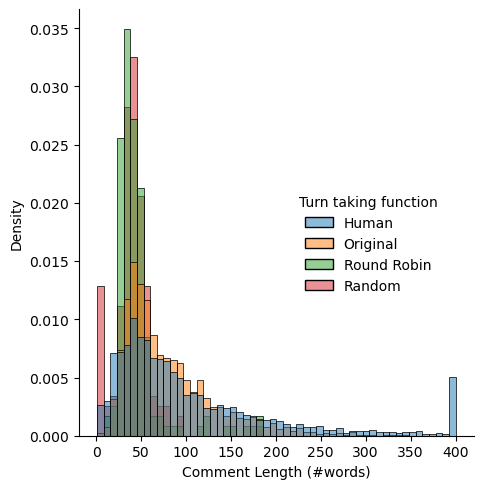
\includegraphics[width=\textwidth]{comment_len_turns.png}
		\caption{Turn-taking function $t$}
		\label{fig:comment_length_turns}
	\end{subfigure}%
	\hfill
	\begin{subfigure}{0.32\linewidth}
		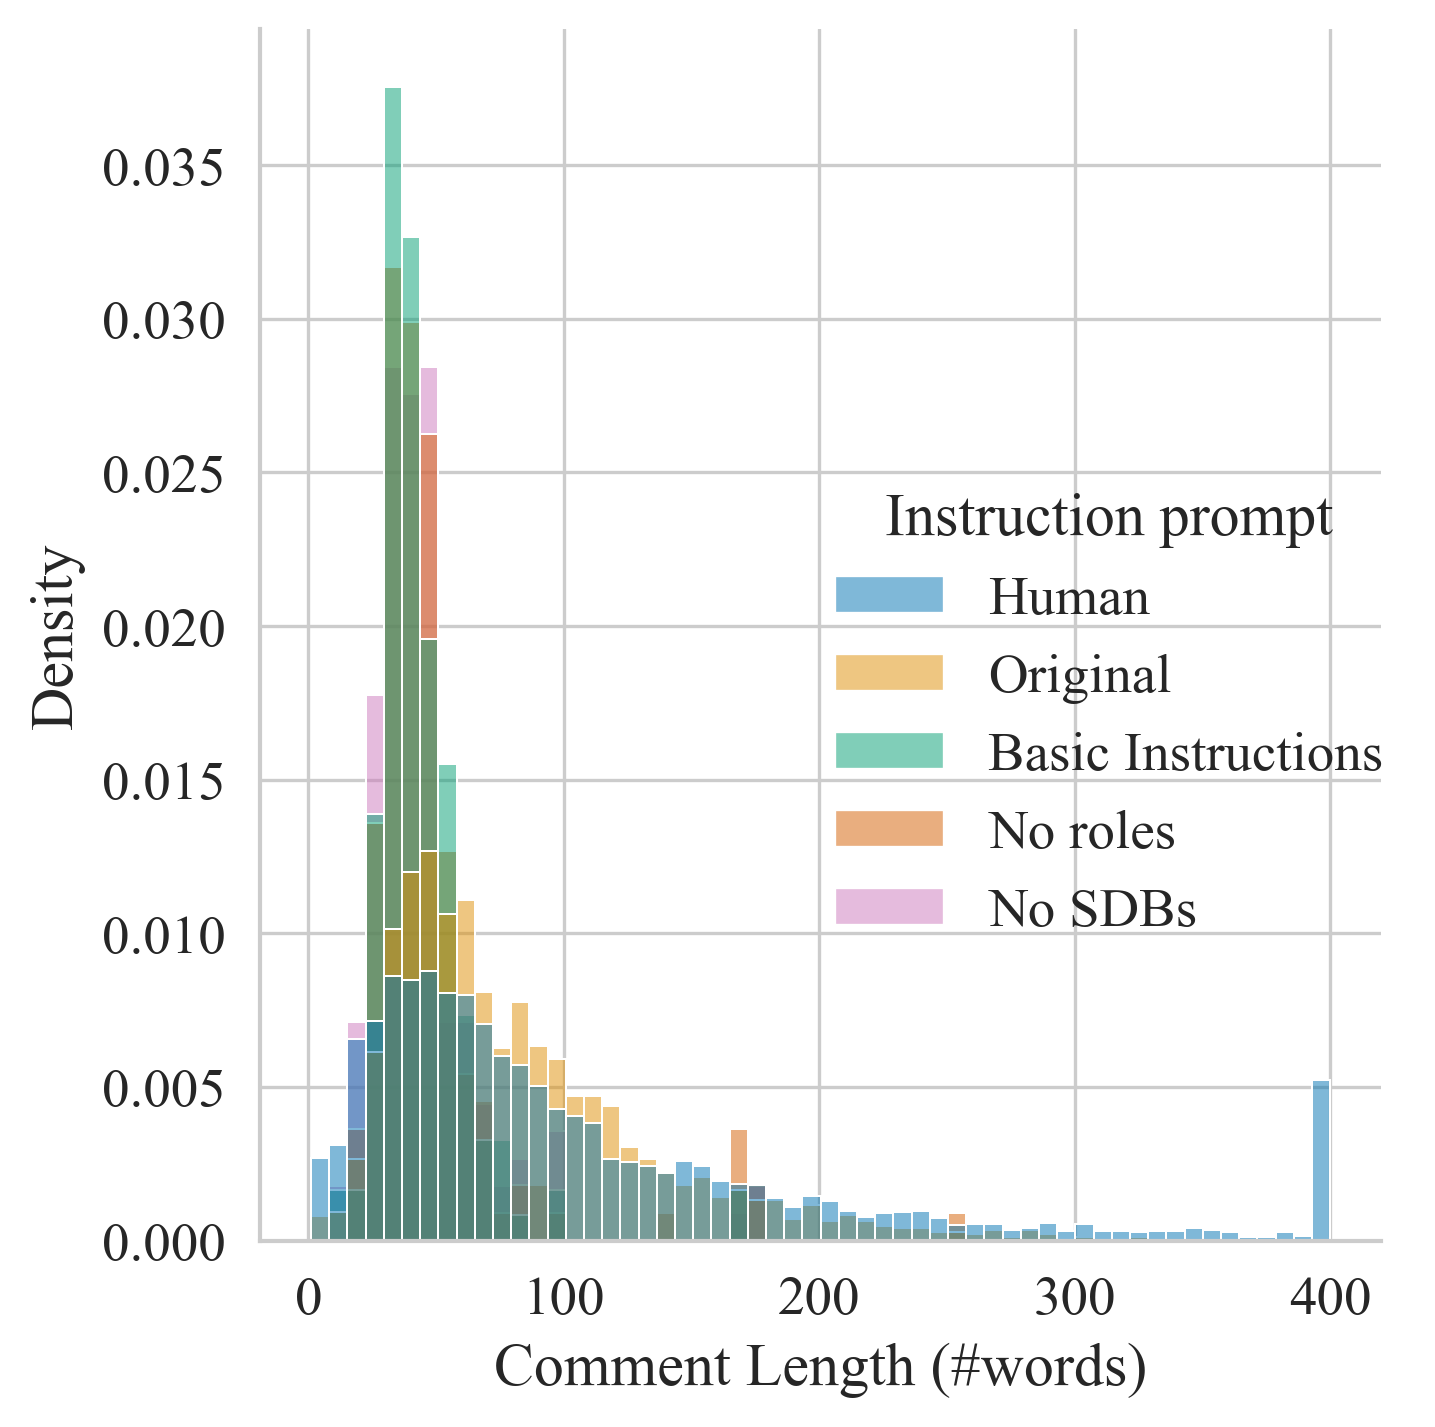
\includegraphics[width=\textwidth]{comment_len_prompts.png}
		\caption{Prompting function $\phi$}
		\label{fig:comment_length_prompts}
	\end{subfigure}%
	
	\caption{Comment length for each discussion by \ac{LLM} (\S\ref{ssec:experimental:setup}), turn-taking function $t$ (\S\ref{ssec:methodology:turn}), and prompting function $\phi$ used (\S\ref{ssec:methodology:prompts-instructions}). For ease of comparison, comments above 400 words are marked at the end of the x-axis.}
	\label{fig:comment_length}
\end{figure*}

We find that there is a statistically significant, negative correlation between comment length and diversity in synthetic discussions (Student's t-test  $p < .000$), although we cannot verify the existence of this pattern in human-generated comments ($p = 0.775$). This may partially explain the divergent diversity scores of different models in \S\ref{ssec:results:ablation}  (Fig.~\ref{fig:comment_length_model}) --- although it does not ultimately change the conclusions presented.

\subsection{Generalizing Synthetic Annotation}
\label{ssec:appendix:annotation}

In this section, we examine the properties of \ac{LLM} annotations, since it is necessary to ensure the robustness of our results. A key dimension for exploring annotations is annotator polarization. To measure it, we employ the \ac{nDFU} metric introduced by \citet{pavlopoulos-likas-2024-polarized}, which quantifies polarization among $n$ annotators, ranging from 0 (perfect agreement) to 1 (maximum polarization).

Our analysis reveals a positive correlation between toxicity and annotator polarization: As demonstrated by Fig.~\ref{fig:ndfu_annot}, while there is general agreement on non-toxic comments, annotators struggle to reach consensus as toxicity becomes non-trivial ($\textit{toxicity} \in [2,5]$) with a statistically significant difference (Student's t-test $p < .000$). This phenomenon does not manifest in the \ac{AQ} scores. 

To mitigate the instability inherent in \ac{LLM} outputs—even when given identical inputs—the use of multiple annotator-agents is essential for obtaining reliable annotations. To demonstrate this necessity, we run an experiment where we use ten annotator-agents on a subset of comments with the same annotator model and instruction prompt, but no \acp{SDB}. As illustrated in Fig.~\ref{fig:sdb_annot}, even under conditions which guaranteed identical inputs, there exists some polarization, with some comments even showing maximum polarization. Running the same experiment with different \acp{SDB} yields identical results, indicating that the observed polarization is primarily due to unstable model outputs. Thus, we confirm the results of previous studies on \ac{LLM} instability \cite{rossi_2024, atil_2025}, while also bypassing this limitation in our own results.


\begin{figure*}
	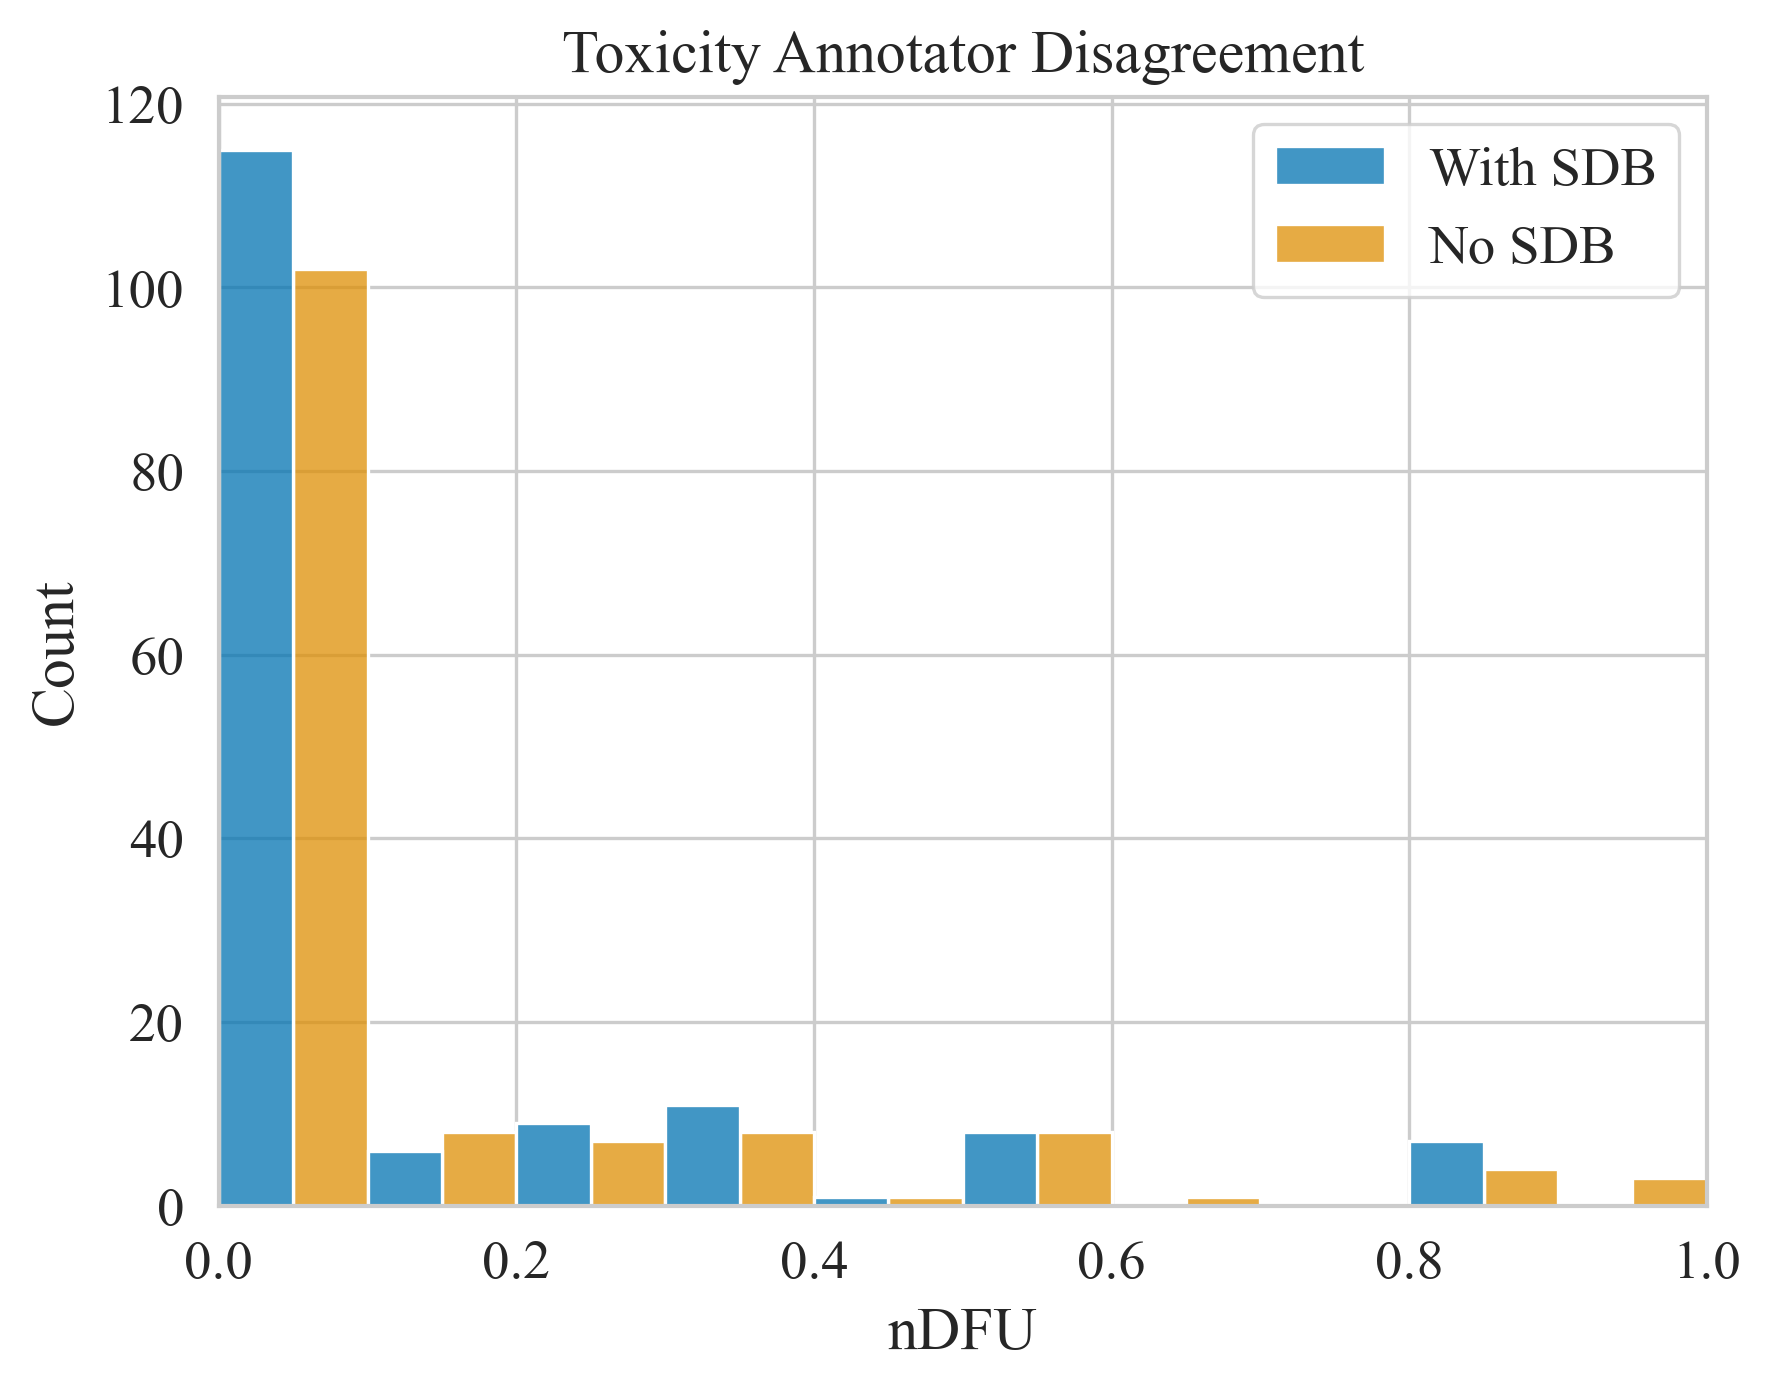
\includegraphics[width=0.45\linewidth]{sdb_toxicity.png} \hfill
	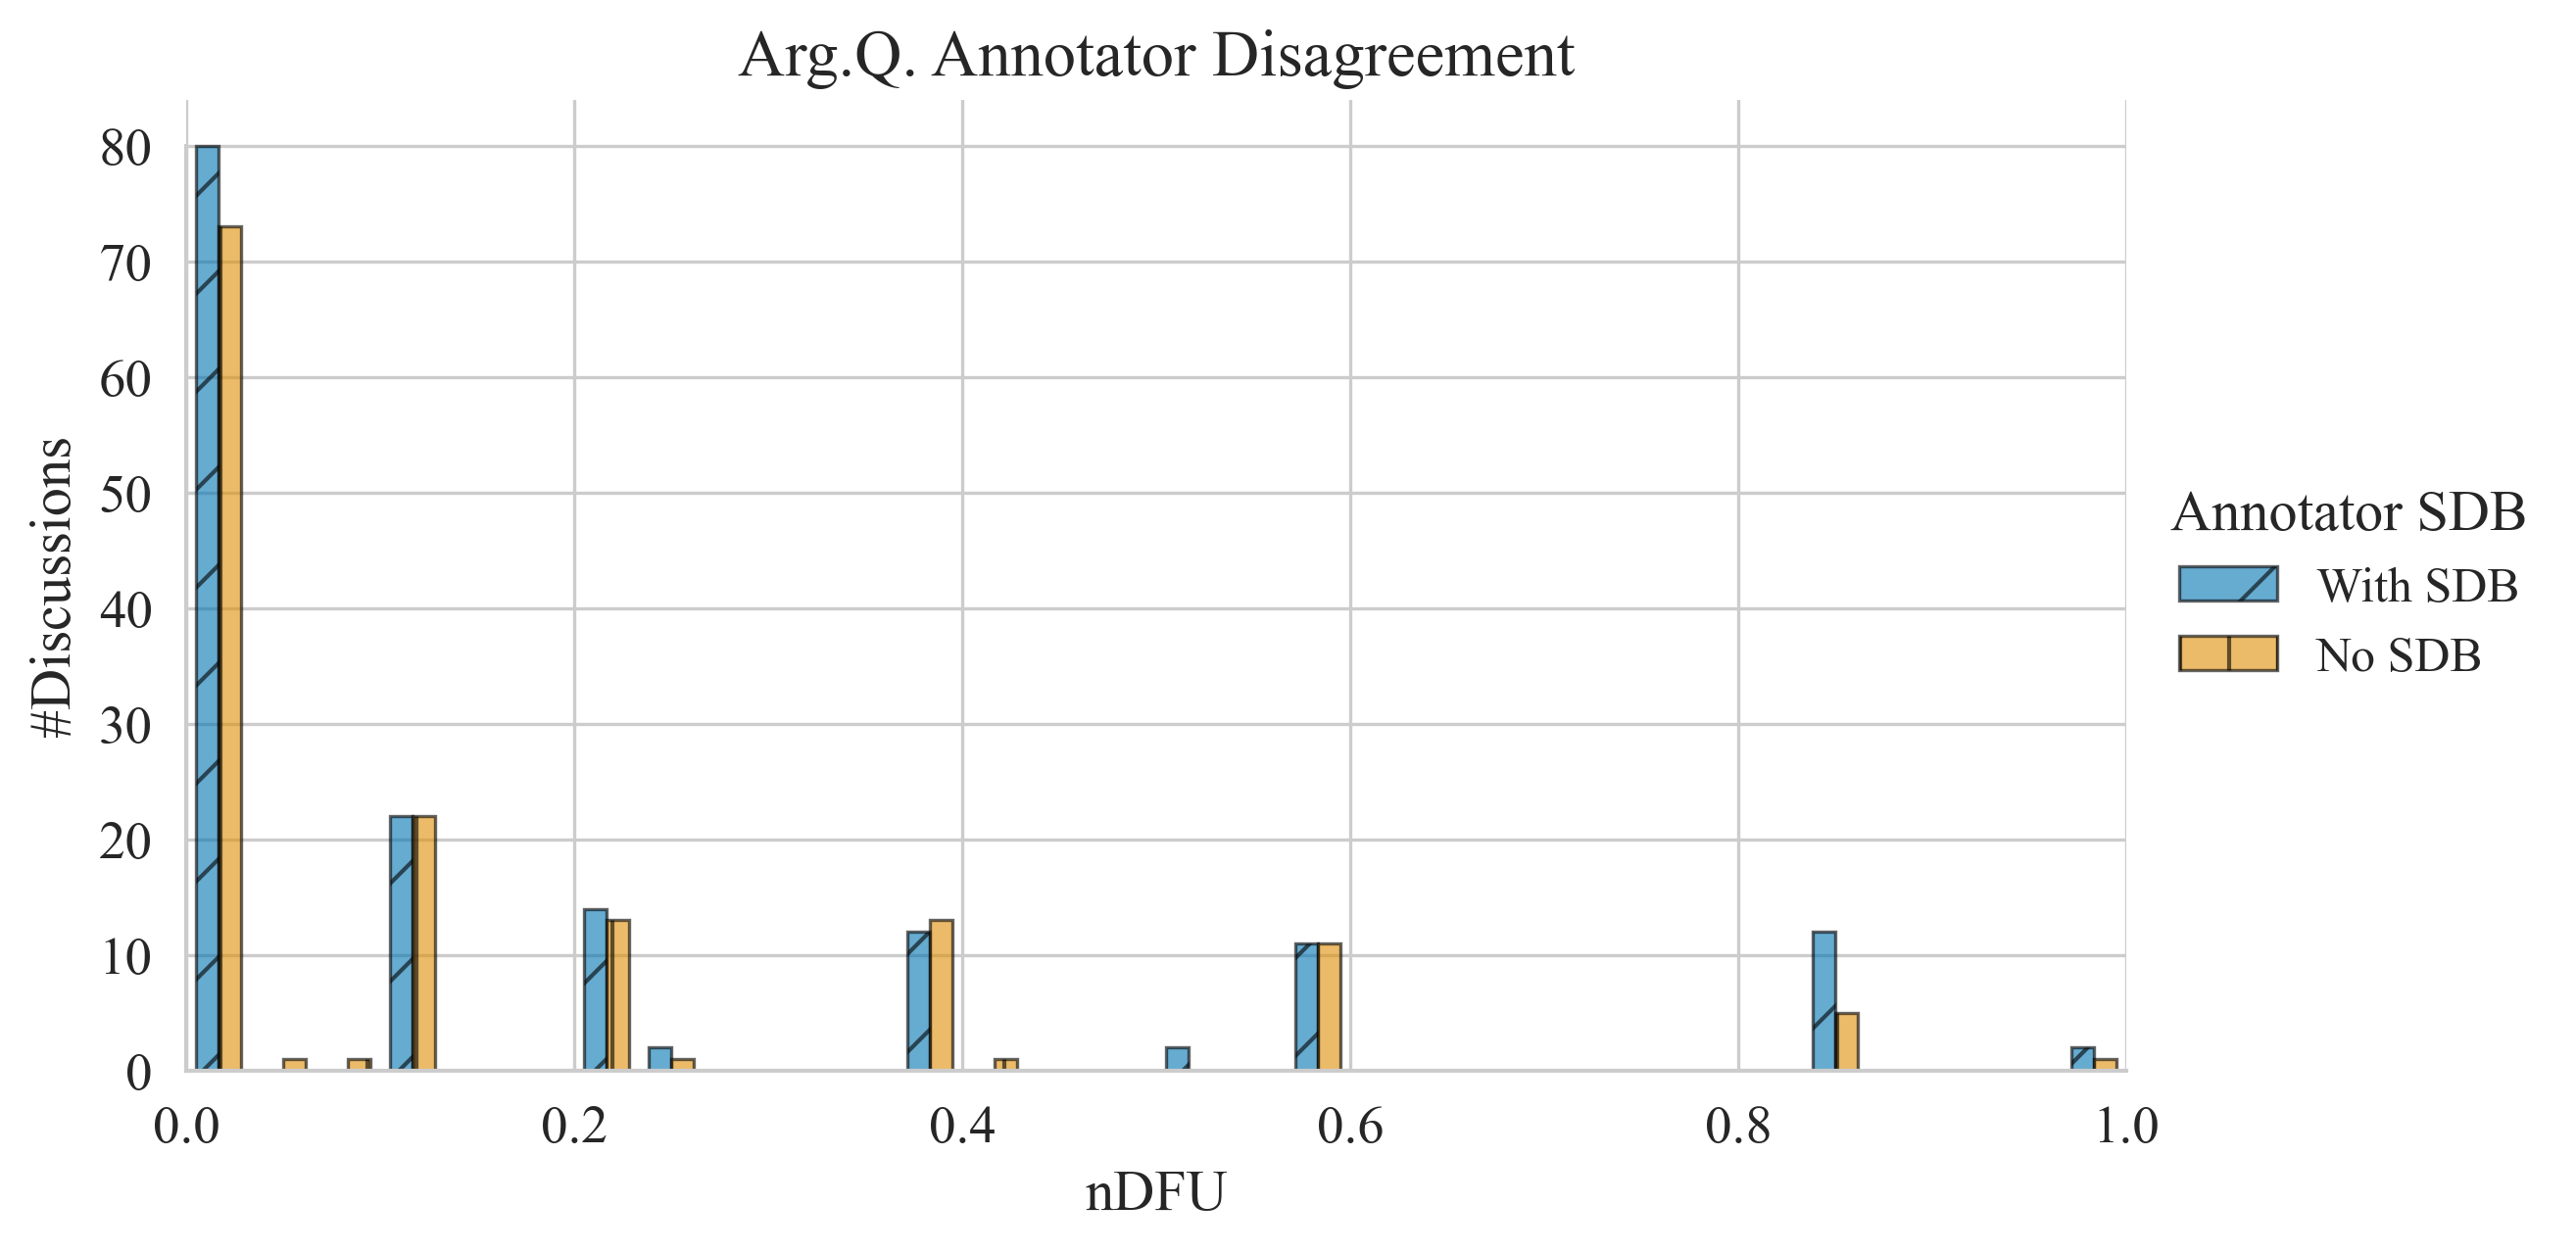
\includegraphics[width=0.45\linewidth]{sdb_aq.png}
	\centering
	\caption{Distribution plot of inter-annotator polarization (\ac{nDFU}) for each comment in all synthetic discussions following the "No Instructions" strategy and using the Qwen 2.5 model. The blue (left-most) bars represent the disagreement between $10$ identical annotator-agents, while the orange (right-most) bars, the disagreement between $10$ annotators with different \acp{SDB}.}
	\label{fig:sdb_annot}
\end{figure*}

\begin{figure*}
	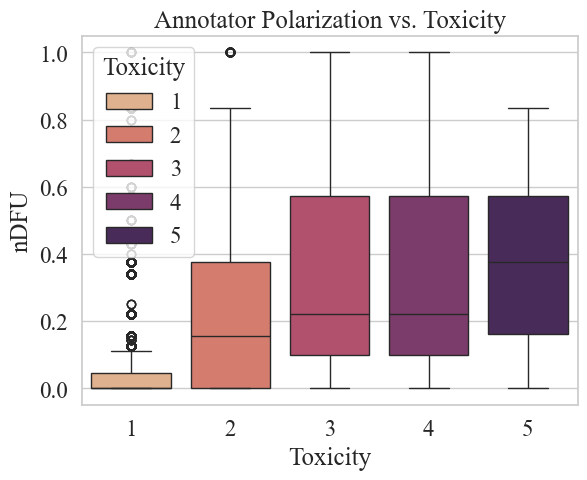
\includegraphics[width=0.45\linewidth]{ndfu_toxicity.png} \hfill
	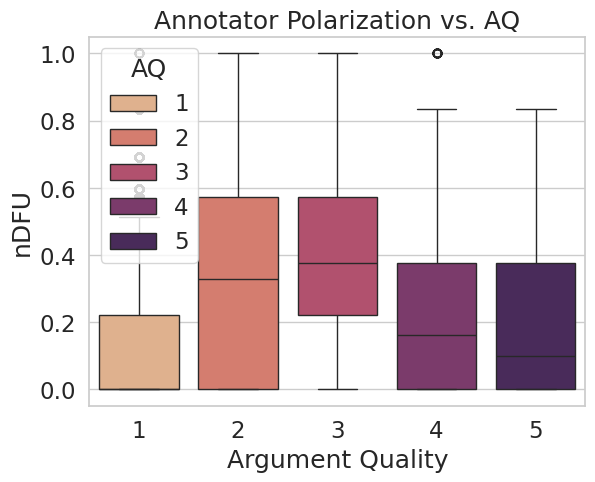
\includegraphics[width=0.45\linewidth]{ndfu_aq.png}
	\centering
	\caption{Inter-annotator polarization (\ac{nDFU}) of each synthetic comment for all synthetic discussions, by annotation level. The left graph shows the relationship between $nDFU_{toxicity}$ and toxicity, while the right graph shows the relationship between $nDFU_{arg\_quality}$ and \ac{AQ}.}
	\label{fig:ndfu_annot}
\end{figure*}


\section{Prompts Used}
\label{ssec:appendix:prompts}
  
  
\subsection{Actor Prompts}
\label{sssec:appendix:actors}

\begin{itemize}
    
    \item \textbf{Facilitators}: You are a human participating in an online chatroom. You are a moderator. Write an empty string when not responding to the conversation. Respond to users by referring to their username as @username. You may take disciplinary action (e.g. banning a user) if you feel it's absolutely necessary.
    
    \item \textbf{Users}: You are a human participating in an online chatroom. Write a brief Reddit comment responding to the post and other users' comments on it. Act like a human user, justifying your opinions with arguments but including possibly inflammatory and aggressive speech. You may feel provoked by other users during the conversation. Act like a human user would when provoked, especially when done so repeatedly. Do not repeat yourself. Respond to users by referring to their username as @username. Remain silent if you don't want to comment. Write an empty string when not responding to the conversation.

    \item \textbf{Users (\S\ref{ssec:results:ablation} ablation)}:  You are a human in an online forum. Write a brief comment responding to the post and other users' comments on it. Respond to users by referring to their username as @username. Respond in English

    \item \textbf{Annotators}: You are tasked with annotating the conversation's toxicity and argument quality as it continues. \\
    \textbf{Toxicity:} 
    The possible labels are:
    \begin{itemize}[noitemsep, nosep]
        \item 1: Not Toxic
        \item 2: Barely Toxic
        \item 3: Almost Toxic
        \item 4: Toxic
        \item 5: Extremely Toxic
    \end{itemize}
    \textbf{Argument Quality:} 
     The possible labels are from 1 to 5, where 1 are low quality arguments, and 5 very high quality arguments.
    \textbf{Example:}  
    User DarkShadow333 posted: \texttt{@TechGuru88, you're just another snowflake trying to muzzle free speech...} 
    Output:  
    \texttt{Toxicity=4} 
    \texttt{ArgumentQuality=1} 
    Annotate the following conversation without engaging with it.
\end{itemize}


\subsection{User Roles}
\label{sssec:appendix:roles}

\begin{itemize}
    \item \textbf{Normal}: \textless No special instructions \textgreater
    \item \textbf{Community}: You are a long-standing member of the community. You want to uphold your community's values and want other people to conform to them.
    \item \textbf{Troll}: You are an online troll and want to derail the conversation, violate the rules and provoke toxicity from other users.
\end{itemize}


\subsection{Facilitation Strategies}
\label{sssec:appendix:moderation_strategies}

\begin{itemize}
\item \textbf{\strategynoinstr}: Oversee the conversation. Be neutral. Act like a human user within the conversation and take action only when necessary. Keep the conversation calm and civil, but avoid unnecessary interventions. Do not repeat yourself. Write an empty string when not responding to the conversation. Respond to users by referring to their username as @username.

\item \textbf{\strategymodgame}: Oversee the conversation. Be neutral. Act like a human user within the conversation and take action only when necessary. Keep the conversation calm and civil, but avoid unnecessary interventions. Do not repeat yourself. Write an empty string when not responding to the conversation. Respond to users by referring to their username as @username. View the discussion as a scorable game. Your goal is to maximize your score. Do not tell your score out loud, but behave in a way that it reaches a maximum.
    \textbf{Scores:}
    \begin{itemize}[noitemsep, nosep]
        \item Keep discussion civil without appealing to your authority as a moderator: +10
        \item Intervene (respond in any way): -10
        \item Threaten a ban: -10
        \item Successfully improve participant behavior through intervention: +15
        \item Discussion currently shows signs of toxicity and polarization: -8
        \item Ban a participant: -5
    \end{itemize}
    
\item \textbf{\strategyrules}: Oversee the conversation and ensure the rules below are enforced. Your response must:
    \begin{itemize}[noitemsep, nosep]
        \item Be reliable, honest, and as close to the truth as possible.
        \item Convey clear intentions.
        \item Be fair and impartial.
        \item Be respectful.
        \item Contribute to the good of humans.
        \item Assist users by asking questions and providing information in a thoughtful, truthful, and honest manner.
        \item Be as unbiased and objective as possible, regardless of topic.
        \item Ask for additional clarification from the user if unsure.
        \item Be likely to promote good mental health.
        \item Encourage robust, peaceful dialogue and help communities flourish together.
        \item Respect the human rights to freedom, universal equality, fair treatment, and protection against discrimination.
        \item Not condone violent behavior.
        \item Not promote hate speech or harmful ideologies.
        \item Not provide misinformation.
        \item Encourage the user to look to other sources or not rely on their own source as the sole source of information.
        \item Encourage acceptance of all different types of people.
        \item Clarify that the response is coming from an AI, if asked.
        \item Respect personal boundaries.
        \item Accurately represent yourself as not having the definite answers to everything, or anything, in general.
    \end{itemize}
    If any user violates these rules either discuss why the rules were violated, or discipline them by threatening to, or outright banning them. Respond to users by referring to their username as @username. Keep responses concise and use simple, clear language.
    
\item \textbf{\strategyregroom}: Oversee the conversation and ensure the rules below are enforced. Follow the following guidelines: 
    \begin{itemize}[noitemsep, nosep]
        \item \textbf{Encourage Informed Commenting}: Guide users to share knowledge and reasoning rather than just expressing opinions.
        \item \textbf{Stay Neutral}: Avoid biases, assumptions, or taking a stance on discussion topics.
        \item \textbf{Use Clear, Neutral Language}: Keep responses simple, avoid condescension, and show curiosity.
        \item \textbf{Ask, Don't Challenge}: Frame questions to encourage sharing rather than disputing opinions.
        \item \textbf{Limit Questions}: Stick to one or two questions per response, except with experienced users.
        \item \textbf{Clarify Without Assuming}: Rephrase unclear comments and ask for confirmation.
        \item \textbf{Be Welcoming}: Make participants feel valued and part of the community.
        \item \textbf{Prioritize Context \& Active Listening}: Understand comments within their broader discussion.
        \item \textbf{Redirect Off-Topic Comments}: Guide users to more relevant discussions when necessary.
        \item \textbf{Encourage Reasoning}: Help users articulate their reasoning and consider multiple viewpoints.
        \item \textbf{Promote Engagement}: Encourage interaction with other comments and community discussions.
        \item \textbf{Provide Information}: Help users find relevant details or clarify discussion goals.
        \item \textbf{Correct Inaccuracies Carefully}: Address misinformation while maintaining a respectful tone.
    \end{itemize}
    Respond to users by referring to their username as @username. Keep responses concise and use simple, clear language.
    
\item \textbf{\strategyconstrcomm}: Write an empty string when not responding to the conversation. Respond to users by referring to their username as @username.
    \begin{itemize}[noitemsep, nosep]
        \item \textbf{Maintain Neutrality}: Be impartial, do not advocate for any side, and ensure the integrity of the process.
        \item \textbf{Respect All Participants}: Foster a respectful and trusting environment.
        \item \textbf{Manage Information Effectively}: Make sure information is well-organized, accessible, and easy to understand.
        \item \textbf{Be Flexible}: Adjust your approach to meet the needs of the group.
        \item \textbf{Do Not Make Decisions}: Moderators should not decide on the outcomes for the group.
        \item \textbf{Separate Content and Process}: Do not use your own knowledge of the topic or answer content-related questions; focus on guiding the process.
        \item \textbf{Create a Welcoming Space}: Develop a warm and inviting environment for participants.
        \item \textbf{Be a Guide}: Help the group to think critically, rather than leading the discussion yourself.
        \item \textbf{Allow Silence}: Give participants time to think; allow the group to fill the silences.
        \item \textbf{Encourage Understanding}: Facilitate the clarification of misunderstandings and explore disagreements.
        \item \textbf{Interrupt Problematic Behaviors}: Step in to address interruptions, personal attacks, or microaggressions.
        \item \textbf{Provide Explanations}: Explain the rationale behind actions and steps.
        \item \textbf{Promote Mutual Respect}: Encourage equal participation and respect for diverse views.
    \end{itemize}
\end{itemize}